%%%%%%%%%%%%%%%%%%%%%%%%%%%%%%%%%%%%%%%%%
% Short Sectioned Assignment
% LaTeX Template
% Version 1.0 (5/5/12)
%
% This template has been downloaded from:
% http://www.LaTeXTemplates.com
%
% Original author:
% Frits Wenneker (http://www.howtotex.com)
%
% License:
% CC BY-NC-SA 3.0 (http://creativecommons.org/licenses/by-nc-sa/3.0/)
%
%%%%%%%%%%%%%%%%%%%%%%%%%%%%%%%%%%%%%%%%%

%----------------------------------------------------------------------------------------
%	PACKAGES AND OTHER DOCUMENT CONFIGURATIONS
%----------------------------------------------------------------------------------------

\documentclass[paper=a4, fontsize=11pt]{scrartcl} % A4 paper and 11pt font size

\usepackage[T1]{fontenc} % Use 8-bit encoding that has 256 glyphs
\usepackage{fourier} % Use the Adobe Utopia font for the document - comment this line to return to the LaTeX default
\usepackage[english]{babel} % English language/hyphenation
\usepackage{amsmath,amsfonts,amsthm} % Math packages

\usepackage{lipsum} % Used for inserting dummy 'Lorem ipsum' text into the template

\usepackage{graphicx}
\usepackage{extarrows}
\usepackage{amssymb}

\usepackage{sectsty} % Allows customizing section commands
\allsectionsfont{\centering \normalfont\scshape} % Make all sections centered, the default font and small caps

\usepackage{fancyhdr} % Custom headers and footers
\pagestyle{fancyplain} % Makes all pages in the document conform to the custom headers and footers
\fancyhead{} % No page header - if you want one, create it in the same way as the footers below
\fancyfoot[L]{} % Empty left footer
\fancyfoot[C]{} % Empty center footer
\fancyfoot[R]{\thepage} % Page numbering for right footer
\renewcommand{\headrulewidth}{0pt} % Remove header underlines
\renewcommand{\footrulewidth}{0pt} % Remove footer underlines
\setlength{\headheight}{13.6pt} % Customize the height of the header

\numberwithin{equation}{section} % Number equations within sections (i.e. 1.1, 1.2, 2.1, 2.2 instead of 1, 2, 3, 4)
\numberwithin{figure}{section} % Number figures within sections (i.e. 1.1, 1.2, 2.1, 2.2 instead of 1, 2, 3, 4)
\numberwithin{table}{section} % Number tables within sections (i.e. 1.1, 1.2, 2.1, 2.2 instead of 1, 2, 3, 4)

\setlength\parindent{0pt} % Removes all indentation from paragraphs - comment this line for an assignment with lots of text

%----------------------------------------------------------------------------------------
%	TITLE SECTION
%----------------------------------------------------------------------------------------

\newcommand{\horrule}[1]{\rule{\linewidth}{#1}} % Create horizontal rule command with 1 argument of height

\title{	
\normalfont \normalsize 
\textsc{National Sun Yat-sen University, Department of Mathematics} \\ [25pt] % Your university, school and/or department name(s)
\horrule{0.5pt} \\[0.4cm] % Thin top horizontal rule
\huge Reliability Analysis Assignment 2 \\(group)\\ % The assignment title
\horrule{2pt} \\[0.5cm] % Thick bottom horizontal rule
}

\author{Chia-Hsuan Chang \ and \ Kuan-I Chung} % Your name

\date{\normalsize 2017.03.20} % Today's date or a custom date

\begin{document}

\maketitle % Print the title

%----------------------------------------------------------------------------------------
%	2.5
%----------------------------------------------------------------------------------------
2.5
\begin{itemize}
	\item[(a)]{
		\begin{align*}
			f(t)	&=	\frac{d}{dt}(1-exp(t)) = exp(-t)\\
			h(t)	&=	\frac{f(t)}{1-F(t)} = \frac{exp(-t)}{1-(1-exp(t))} = 1
		\end{align*}
	}
	
	\item[(b)]{\
		\begin{figure}[h]
			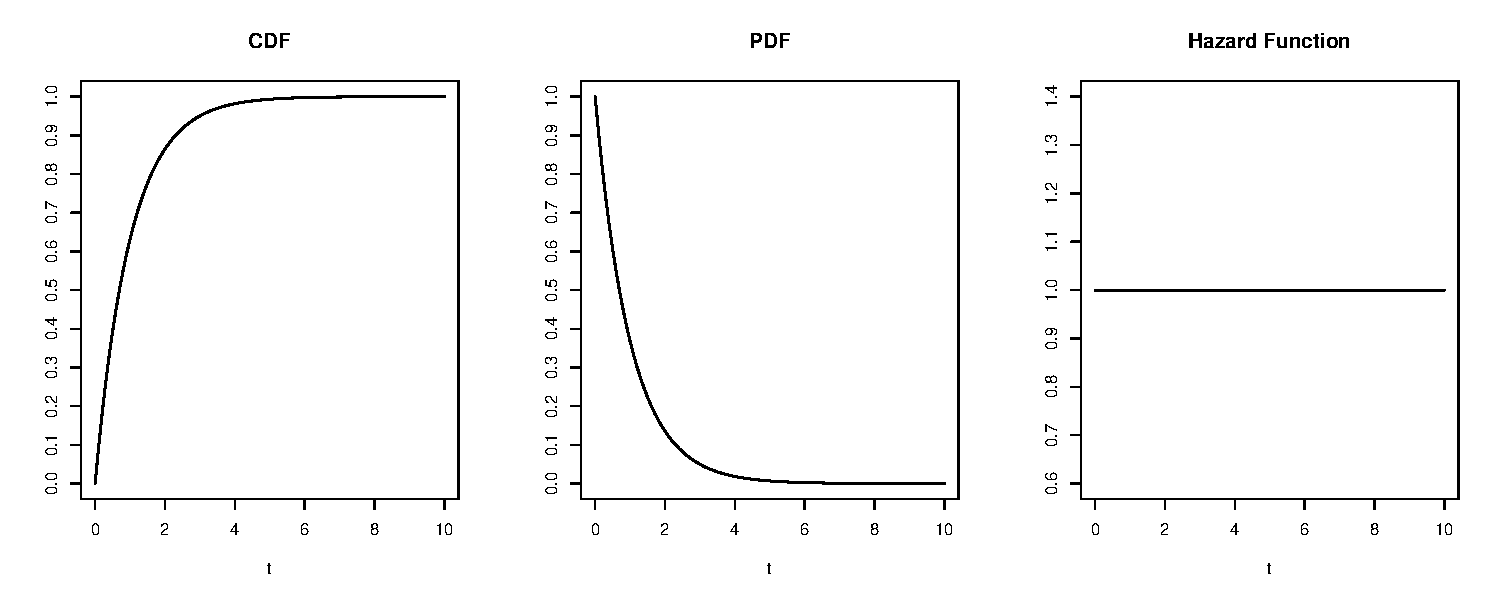
\includegraphics[width = 5.5 in]{2_5_b.pdf}
		\end{figure}

	}
	
	\item[(c)]{
		\begin{align*}
						&	F(t_p) = p = 1-exp(-t_p)\\
			\Rightarrow	&	exp(-t_p) = 1-p\\
			\Rightarrow	&	-t_p = log(1-p)	\\
			\Rightarrow	&	t_p = -log(1-p) \\
			\Rightarrow	&	t_{.1} = -log(1-0.1) = -log(0.9) \approx 0.1054
		\end{align*}
		\begin{figure}[h]
			\centering
			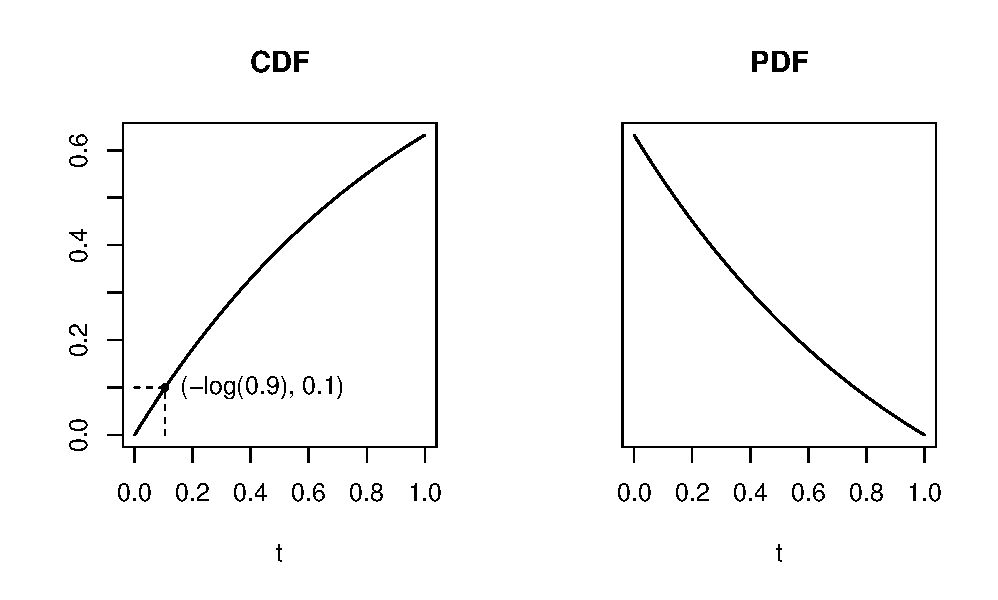
\includegraphics[width = 3.8 in]{2_5_c.pdf}
		\end{figure}
	}
	
	\item[(d)]{
		\begin{align*}
						&	Pr(0.1 < T \leq 0.2) = F(0.2) - F(0.1) = exp(-0.1) - exp(-0.2) \approx 0.0861\\
			\Rightarrow\ \ 	&	Pr(0.1 < T \leq 0.2 \vert T>0.1) = \frac{F(0.2) - F(0.1) }{1 - F(0.1) } 
							= \frac{ exp(-0.1) - exp(-0.2)}{ exp(-0.1)} \approx  0.0952
		\end{align*}	
		\	
		\begin{figure}[h]
			\centering
			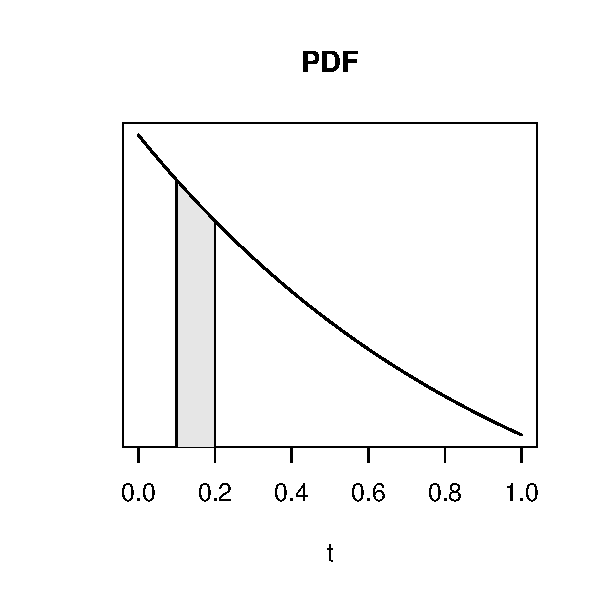
\includegraphics[width = 2.3 in]{2_5_d.pdf}
		\end{figure}
		%\begin{equation*}
			\\ $\qquad \ \ \ \ \ \ \ \ \  h(0.1) \cdot (0.2-0.1) = 0.1 \approx 0.0952$
		%\end{equation*}
	}
\end{itemize}

%----------------------------------------------------------------------------------------
%	2.6
%----------------------------------------------------------------------------------------
2.6
\begin{itemize}
	\item[(a)]{\
		\begin{figure}[h]
			\centering
			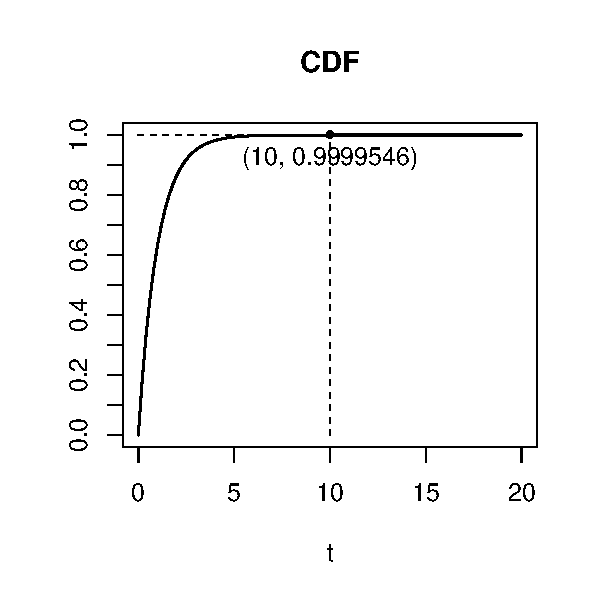
\includegraphics[width = 2.3 in]{2_6_a.pdf}
		\end{figure}	
	}
	
	\item[(b)]{\ \\ 
		\begin{tabular}{c | rrrr}
			$t_i$		&	$F(t_i)$		&	$S(t_i)$	&	$\pi(t_i)$	&	$p_i$ 	\\ \hline
			0.1 		&	0.0952 		&	0.9048 	&	0.0952 	&	0.0952	\\
			0.2 		&	0.1813 		&	0.8187 	&	0.0861 	&	0.0952	\\
			0.5 		&	0.3935 		&	0.6065 	&	0.2122 	&	0.2592	\\
			1 		&	0.6321 		&	0.3679	&	0.2387 	&	0.3935	\\
			2 		&	0.8647 		&	0.1353 	&	0.2325 	&	0.6321	\\
			$\infty$ 	&	1.0000 		&	0.0000 	&	0.1353 	&	1.0000	\\
		\end{tabular}
	}
\end{itemize}

%----------------------------------------------------------------------------------------
%	2.8
%----------------------------------------------------------------------------------------
2.8\\
\qquad 
$
	L(p) =  	C\left( (F(8))^0 (1-F(8))^{39}\cdot (F(12)-F(8))^4\ (1-F(12))^{49}\cdots 
			(F(44)-F(40))^{21} \ (1-F(44))^{19+21+15}\right)
$
If we know the exact event time, the likelihood function will consist the term of $f(t_i)$. \\ \ \\
%----------------------------------------------------------------------------------------
%	2.9
%----------------------------------------------------------------------------------------
2.9
\begin{itemize}
	\item[(a)]{
		Because we do not know when the samples had been existing before the experiment, the failures in the interval $0-25$ days could be considered to be left-censored observation.
	}
	
	\item[(b)]{
		Because we do not know when the samples would fail after the end of the experiment, the failures in the interval $100-\infty$ days could be considered to be left-censored observation.

	}
\end{itemize}
%----------------------------------------------------------------------------------------
%	2.10
%----------------------------------------------------------------------------------------
2.10\\
$
	L(p) =  	C\left( (F(25))^{109}\  (F(50)-F(25))^{42}\ (F(75)-F(50))^{17}\ (F(100)-F(75))^{7} \ 
			(1-F(100))^{13} \right)
$

%----------------------------------------------------------------------------------------

\end{document}